\section{EXPERIMENTAL RESULTS}

We will next empirically compare the capacity of the qNML to that of
BIC, BDeu and fNML in identifying the data generating structures,
and producing models that are predictive and parsimonious.
It seems that none of the criteria outperform others for all
these requirements. 

\subsection{FINDING GENERATING STRUCTURE}

We first compared the ability of different scoring criteria to
discover the data generating structure. For this purpose we generated
100 different 5-node Bayesian network structures with 4 edges and
another 100 structures with 7 edges.  The variables were randomly
assigned to have 2 – 4 values ($r_i \in \{2, 3, 4\}$). For each
network, we generated parameters by two different schemes. The first
scheme exactly matched the assumptions of the BDeu score with $\alpha
= 1$, i.e., the parameters were distributed by $\theta_{ij} \sim
Dir(\frac{1}{r_iq_i},\ldots,\frac{r_i}{q_i})$. The other scheme was
to generate the parameters independently from a Dirichlet distribution
$\theta_{ij} \sim Dir(\frac{1}{2},\ldots, \frac{1}{2})$ that is the
Jeffreys' prior for multinomial model. This distribution was selected
instead of the uniform distribution in order to make the generating
structure more identifiable.  For each network (structure +
parameters), we generated 100 data sets of 1000 data vectors, and
studied how different scoring criteria ranked the structure of the
generating network among all the 5-node networks as a function of
(sub)sample size.

Not surprisingly, the results indicate that when the parameter generation
mechanism matches the assumptions of the BDeu-score, the BDeu usually
also ranks the generating structure higher than the other scores
(Figure X).  On the other hand, when the paramaters are drawn from the
Jeffreys's prior, the fNML score appears to rank the generting structure
highest. This too is not surprising, since the NML distribution for the
multinomial data is known to closely match the marginal distribution of
the data when the Jefrreys' prior is used (CITE).

The underfitting tendency of BIC can also be clearly detected both for
relatively sparse networks (4 arcs) and the dense ones (7 arcs). The
ranking ability the qNML criterion appears to be between fNML and BDeu
in 3 out of for settings which is good considering that one of these
criteria is always the winner. For the dense networks with BDeu prior,
the qNML appears to perform worse than BDeu and fNML but still much
better than BIC.

\subsection{PREDICTION AND PARSIMONY}

To empirically compare the model selection criteria we took 20 UCI
data sets~\cite{Lichman:2013} and run 1000 train and test experiments
for 20 different sample sizes for all of them. The training was
conducted using a dynamic programming based exact structure
learning~\cite{cosco.uai06} which limited the number $n$ of variables
to less than 20.

Figure~\ref{fig:bcmean} shows an example of the behavior of the
studied selection criteria.  For small sample sizes fNML and qNML
yield equally accurate predictions while BDeu requires more samples to
obtain competitive performance. The curves are mean curves from 1000
independent train and test splits.

\begin{figure}
\centering
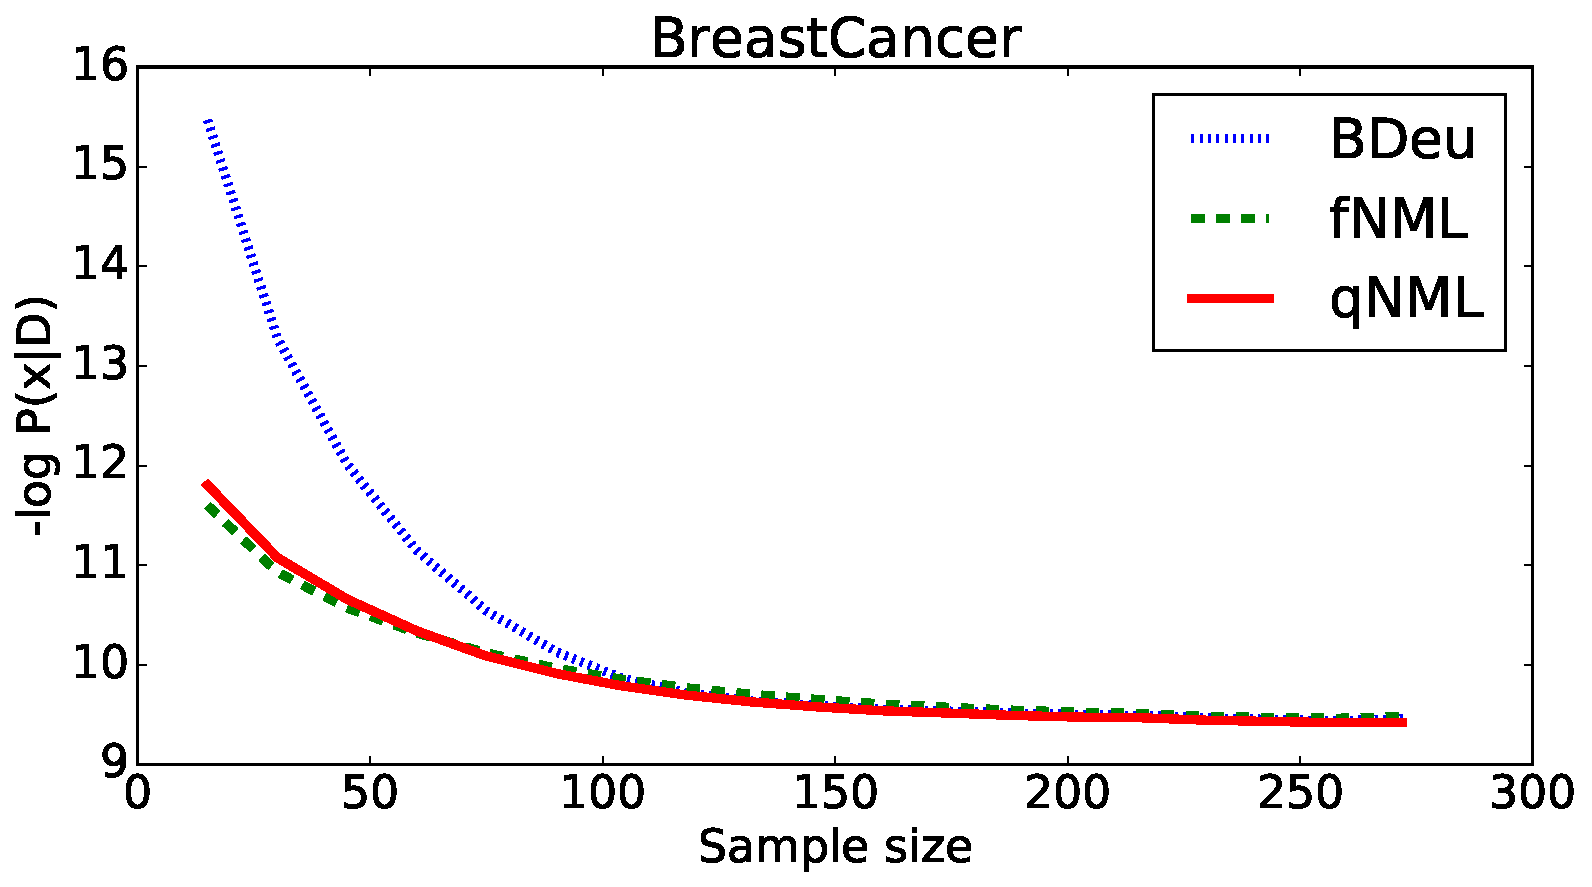
\includegraphics[width=8cm,height=5cm]{breast_cancer_mean.pdf}
\caption{Predictive log-loss in a breast cancer data as a function of
  sample size for different model selection criteria.}
\label{fig:bcmean}
\end{figure}

Figure~\ref{fig:bcnpmean} shows how fNML still sometimes behaves
strangely in terms of model complexity here measured by the number of
parameters in the model.  qNML, instead, appears to yield more
parsimonious models.

\begin{figure}
\centering
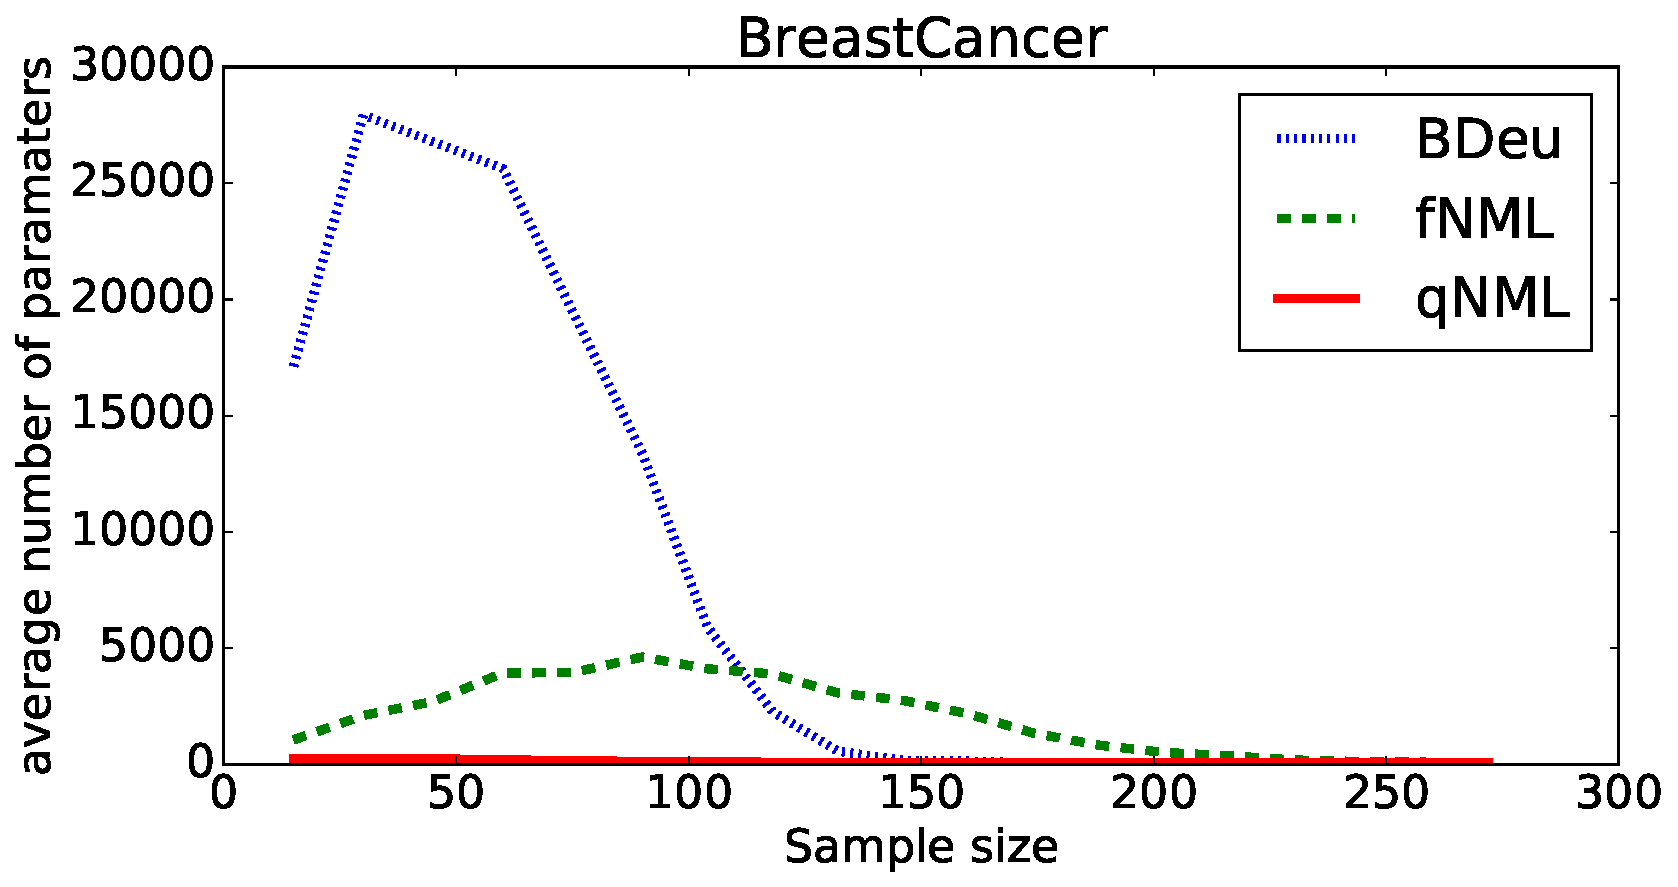
\includegraphics[width=8cm,height=5cm]{breast_cancer_np_mean.pdf}
\caption{Number of parameters in a breast cancer model as a function
  of sample size for different model selection criteria.}
\label{fig:bcnpmean}
\end{figure}

\begin{table}
\centering
\begin{tabular}{crrrr}
\toprule
           Data &     N &   BDeu &            fNML &            qNML \\
\midrule
           Iris &    16 &   3.59 &            3.47 &   \textbf{3.43} \\
  PostOperative &    20 &  10.24 &   \textbf{8.27} &            8.32 \\
           Wine &    27 &  18.11 &           12.68 &  \textbf{12.51} \\
 HeartHungarian &    45 &  10.15 &            9.10 &   \textbf{8.90} \\
   BreastCancer &    45 &  12.01 &  \textbf{10.57} &           10.66 \\
 HeartCleveland &    48 &  16.36 &           12.81 &  \textbf{12.54} \\
          Ecoli &    51 &   5.77 &   \textbf{5.30} &            5.37 \\
          Liver &    54 &   4.07 &            3.97 &   \textbf{3.91} \\
          Glass &    55 &   7.16 &   \textbf{6.22} &            6.28 \\
        Thyroid &    55 &   2.83 &   \textbf{2.75} &            2.77 \\
   HeartStatlog &    56 &  14.15 &           11.92 &  \textbf{11.60} \\
      TicTacToe &    96 &  10.99 &  \textbf{10.73} &           11.05 \\
        Balance &    96 &   7.48 &   \textbf{7.39} &            7.78 \\
    BcWisconsin &   105 &   5.81 &            5.12 &   \textbf{5.08} \\
       Diabetes &   117 &   4.95 &            4.95 &   \textbf{4.89} \\
          Yeast &   225 &   5.54 &   \textbf{5.40} &            5.42 \\
        Abalone &   418 &   3.93 &   \textbf{3.88} &            3.96 \\
     PageBlocks &   548 &   2.36 &   \textbf{2.32} &            2.38 \\
        Shuttle &  2900 &   1.70 &   \textbf{1.69} &            1.72 \\
          Adult &  4885 &  10.22 &  \textbf{10.08} &           10.12 \\
\bottomrule
\end{tabular}
\caption{Predictive log losses for small sample sizes for different model selection criteria in 20 different datasets.}
\label{tbl:preds}
	\end{table}

Table~\ref{tbl:preds} features predictive losses for the small sample
sizes.  (The results for large sample sizes converge for all sensible
criteria.)  As we can see, fNML still usually (12/20) performs best
but qNML is not much worse while BDeu may sometimes perform much
worse.

Looking at the number of parameters for the same datasets and sample
sizes (Table~\ref{tbl:nofparams}) reveals that qNML usually (18/20)
yields simplest models, and sometimes, like in the BreastCancer data,
the differences are of orders of magnitude.

\begin{table}
\centering
\begin{tabular}{crrrr}
\toprule
           Data &     N &          BDeu &  fNML &          qNML \\
\midrule
           Iris &    16 &            36 &    33 &   \textbf{28} \\
  PostOperative &    20 &          1304 &   464 &  \textbf{115} \\
           Wine &    27 &         11559 &   780 &  \textbf{214} \\
 HeartHungarian &    45 &          4706 &   838 &  \textbf{100} \\
   BreastCancer &    45 &         26774 &  2710 &  \textbf{246} \\
 HeartCleveland &    48 &         29346 &  1407 &  \textbf{204} \\
          Ecoli &    51 &           113 &   167 &   \textbf{80} \\
          Liver &    54 &            40 &    60 &   \textbf{24} \\
          Glass &    55 &          1488 &   572 &  \textbf{100} \\
        Thyroid &    55 &            37 &    70 &   \textbf{28} \\
   HeartStatlog &    56 &         18414 &  1099 &  \textbf{159} \\
      TicTacToe &    96 &         13645 &  2438 &  \textbf{696} \\
        Balance &    96 &   \textbf{20} &   237 &           168 \\
    BcWisconsin &   105 &          5921 &   816 &   \textbf{88} \\
       Diabetes &   117 &            35 &   216 &   \textbf{34} \\
          Yeast &   225 &   \textbf{78} &   307 &            80 \\
        Abalone &   418 &            90 &   156 &   \textbf{62} \\
     PageBlocks &   548 &           699 &   377 &   \textbf{56} \\
        Shuttle &  2900 &           380 &   594 &  \textbf{111} \\
          Adult &  4885 &  \textbf{599} &  1431 &           876 \\
\bottomrule
\end{tabular}
\caption{Number of model parameters for small sample sizes for different model selection criteria in 20 different datasets.}
\label{tbl:nofparams}
\end{table}
